% =====================================================================
%  Poly Citra CoolBrick  —  Project Rebrick v2
%  Slide version of the A4 report (classrooms, SDGs 4/11/12/13).
%
%  Compile:  pdflatex poly_citra_coolbrick.tex   (run twice)
%  Needs:    beamer + metropolis theme, pgfplots, tikz, tcolorbox, booktabs
%
%  Anything in \todo{...} is a placeholder the team should fill in or
%  verify with its own measurements before submission.
% =====================================================================
\documentclass[aspectratio=169,10pt]{beamer}

\usetheme[progressbar=frametitle,numbering=fraction,block=fill]{metropolis}
\usepackage[T1]{fontenc}
\usepackage{lmodern}
\usepackage{graphicx}
\usepackage{booktabs}
\usepackage{tabularx}
\usepackage{amsmath}
\usepackage{siunitx}
\usepackage{tikz}
\usetikzlibrary{arrows.meta,positioning,shapes.geometric,calc,decorations.pathmorphing,patterns}
\usepackage{pgfplots}
\pgfplotsset{compat=1.18}
\usepackage[most]{tcolorbox}

\graphicspath{{img/}}

% ---------- palette (matches the original deck: orange + green) ----------
\definecolor{citrus}{HTML}{E8731A}
\definecolor{leaf}{HTML}{2E7D32}
\definecolor{sky}{HTML}{1E88C8}
\definecolor{plum}{HTML}{8E2A8E}
\definecolor{ink}{HTML}{1F2A36}
\definecolor{paper}{HTML}{FAFAF7}
\definecolor{heat}{HTML}{C62828}

\setbeamercolor{frametitle}{bg=ink,fg=white}
\setbeamercolor{progress bar}{fg=citrus,bg=citrus!20}
\setbeamercolor{title separator}{fg=citrus}
\setbeamercolor{normal text}{fg=ink,bg=paper}
\setbeamercolor{alerted text}{fg=citrus}
\setbeamercolor{example text}{fg=leaf}
\setbeamercolor{block title}{bg=leaf!15,fg=leaf!70!black}
\setbeamercolor{block body}{bg=leaf!5}
\setbeamercolor{block title alerted}{bg=citrus!18,fg=citrus!70!black}
\setbeamercolor{block body alerted}{bg=citrus!5}

\newcommand{\todo}[1]{\textcolor{heat}{\textbf{[#1]}}}
\newcommand{\new}{\tikz[baseline=-0.6ex]\node[fill=citrus,text=white,font=\tiny\bfseries,rounded corners=2pt,inner sep=2pt]{NEW};}
\newcommand{\src}[1]{\par\vfill{\tiny\color{gray}Source: #1}}

\newtcolorbox{card}[2][]{enhanced,colback=white,colframe=#2,boxrule=0pt,
  leftrule=3pt,arc=2pt,left=5pt,right=5pt,top=3pt,bottom=3pt,
  fontupper=\small,#1}

\newcommand{\rupeesym}{Rs\,}
\newtcolorbox{usp}{enhanced,colback=citrus!8,colframe=citrus,boxrule=1.2pt,arc=4pt,
  left=8pt,right=8pt,top=8pt,bottom=6pt,title={\bfseries OUR USP},fonttitle=\scriptsize,
  coltitle=white,colbacktitle=citrus,attach boxed title to top left={yshift=-2mm,xshift=8pt},
  boxed title style={arc=2pt,boxrule=0pt}}

\title{Poly Citra \textcolor{citrus}{Cool}Brick}
\subtitle{A brick made from Styrofoam and orange peel that keeps classrooms cool}
\author{Rian Sikka \& Daiwik Abrol}
\institute{Scottish High International School \quad\textbar\quad Grade 9 (IGCSE)}
\date{}
\titlegraphic{\vspace*{0.3cm}\hfill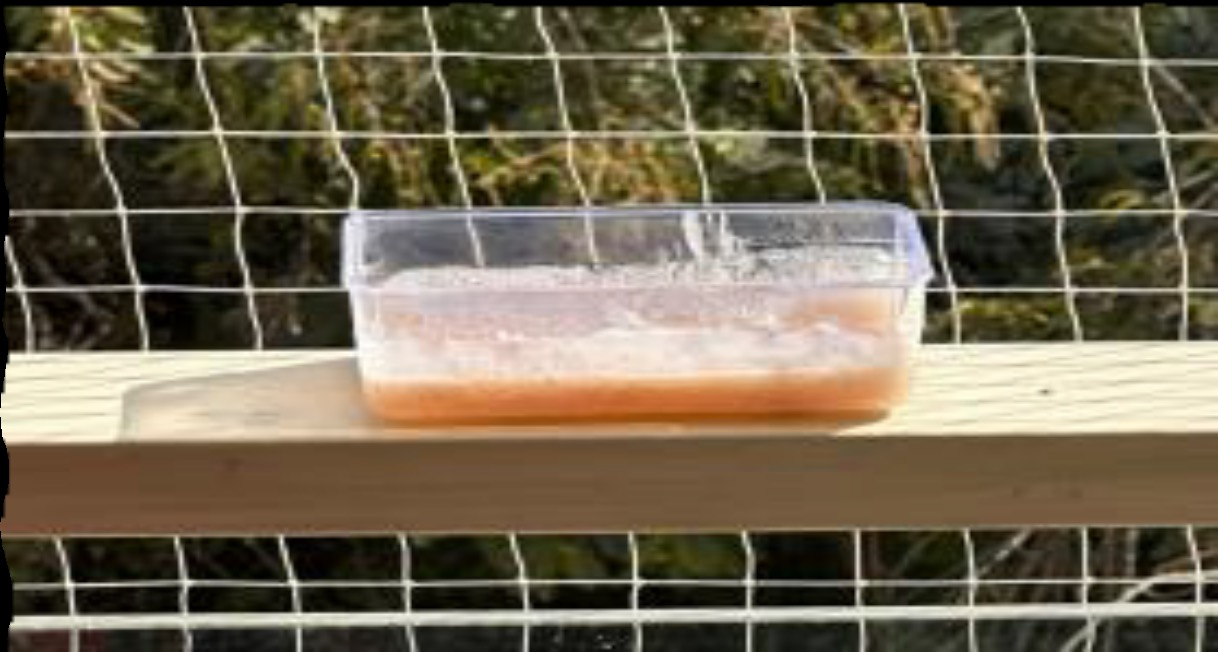
\includegraphics[height=2.3cm]{prototype.jpg}}


\begin{document}
\maketitle

\begin{frame}{The problem}
\begin{columns}[T]
\column{0.52\textwidth}
\begin{itemize}
  \item \textbf{Two wastes.} Styrofoam fills landfills; orange peel from juice shops is dumped or burned.
  \item \textbf{Clay bricks} use fertile topsoil and coal-fired kilns.
  \item \textbf{Hot classrooms.} About 10 lakh government schools in India, most without AC. Every extra \SI{1}{\degree F} of heat cuts learning by about 1\% in schools without AC.
\end{itemize}
\column{0.44\textwidth}
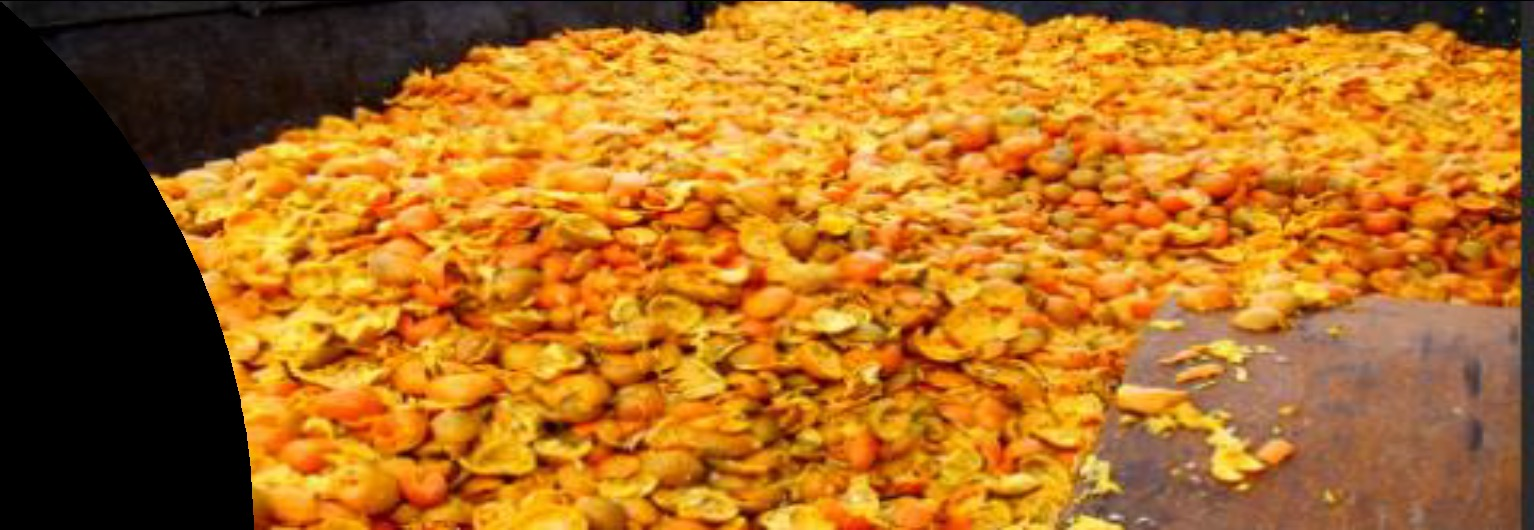
\includegraphics[width=\linewidth,height=2.1cm]{peel-waste.jpg}\\[3pt]
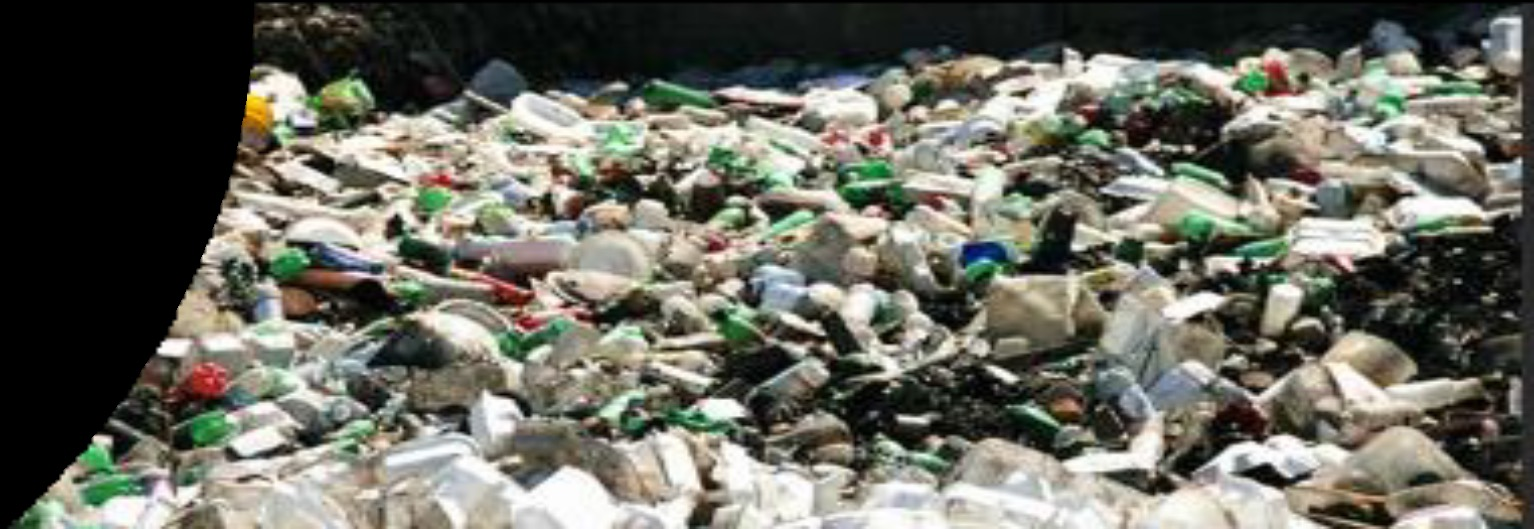
\includegraphics[width=\linewidth,height=2.1cm]{plastic-waste.jpg}
\end{columns}
\end{frame}

\begin{frame}{Our USP}
\vfill
\begin{usp}
\Large\bfseries A brick that keeps rooms cool without electricity, made from two wastes
(Styrofoam and orange peel) instead of mined clay and a coal-fired kiln.
\end{usp}
\vfill
\begin{columns}[T]
\column{0.32\textwidth}\begin{card}{sky}\textbf{80\% less heat}\\ gets in than through clay walls\end{card}
\column{0.32\textwidth}\begin{card}{leaf}\textbf{2 wastes}\\ no kiln, no topsoil\end{card}
\column{0.32\textwidth}\begin{card}{citrus}\textbf{about \rupeesym29}\\ per brick, made in bulk\end{card}
\end{columns}
\vfill
\end{frame}

\begin{frame}{Version 1: Poly Citra Bricks}
\begin{columns}[T]
\column{0.5\textwidth}
\begin{enumerate}
  \item Steam-distil orange peel to get \textbf{D-limonene}.
  \item Limonene dissolves Styrofoam (98\% air) into a thick gel.
  \item Mix with sand, mould and cure. The plastic sets hard.
\end{enumerate}
\medskip
Light, waterproof, no kiln. Recognised at national competitions \todo{awards}.
\column{0.46\textwidth}
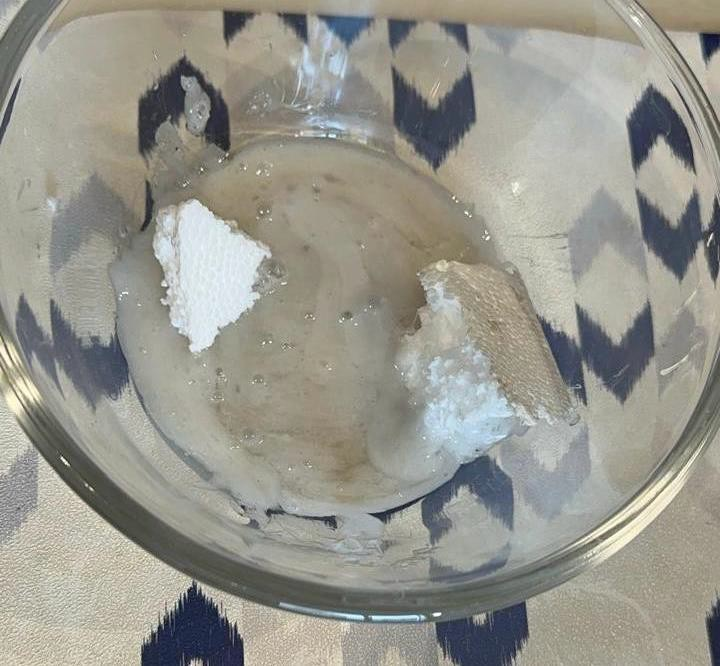
\includegraphics[width=0.49\linewidth,height=2.4cm]{dissolving.jpg}\hfill
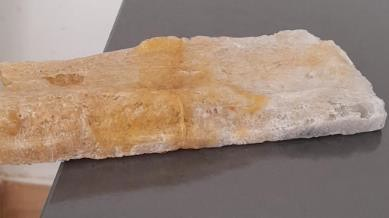
\includegraphics[width=0.49\linewidth,height=2.4cm]{brick-sample.jpg}\\[3pt]
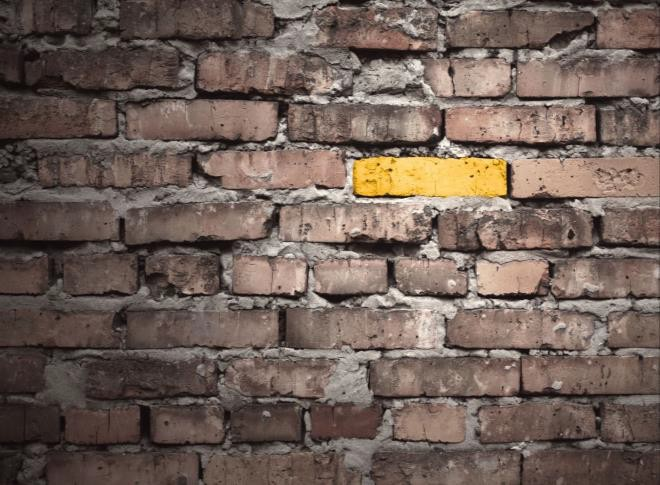
\includegraphics[width=\linewidth,height=2.6cm]{brickwall.jpg}
\end{columns}
\end{frame}

\begin{frame}{Version 2: the CoolBrick}
\begin{columns}[c]
\column{0.5\textwidth}
\centering
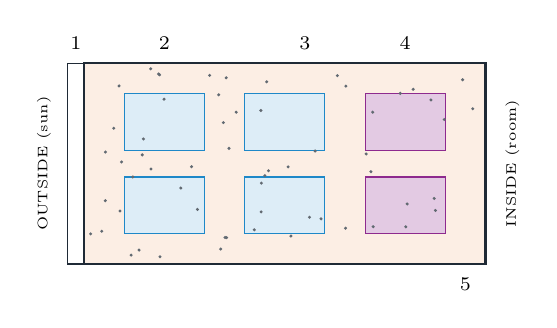
\begin{tikzpicture}[scale=0.85]
  \fill[citrus!12] (0,0) rectangle (6,3); \draw[ink,line width=0.8pt] (0,0) rectangle (6,3);
  \fill[white] (-0.25,0) rectangle (0,3); \draw[ink] (-0.25,0) rectangle (0,3);
  \foreach \x in {0.6,2.4}{\fill[sky!15] (\x,0.45) rectangle ++(1.2,0.85); \draw[sky] (\x,0.45) rectangle ++(1.2,0.85);
                           \fill[sky!15] (\x,1.7) rectangle ++(1.2,0.85); \draw[sky] (\x,1.7) rectangle ++(1.2,0.85);}
  \fill[plum!25] (4.2,0.45) rectangle ++(1.2,0.85); \draw[plum] (4.2,0.45) rectangle ++(1.2,0.85);
  \fill[plum!25] (4.2,1.7) rectangle ++(1.2,0.85); \draw[plum] (4.2,1.7) rectangle ++(1.2,0.85);
  \pgfmathsetseed{7}\foreach \i in {1,...,60}{\fill[ink!70] ({0.1+5.8*rnd},{0.08+2.84*rnd}) circle (0.025);}
  \node[font=\tiny,rotate=90] at (-0.6,1.5) {OUTSIDE (sun)}; \node[font=\tiny,rotate=90] at (6.4,1.5) {INSIDE (room)};
  \node[font=\scriptsize] at (-0.12,3.3) {1}; \node[font=\scriptsize] at (1.2,3.3) {2};
  \node[font=\scriptsize] at (3.3,3.3) {3}; \node[font=\scriptsize] at (4.8,3.3) {4}; \node[font=\scriptsize] at (5.7,-0.3) {5};
\end{tikzpicture}
\column{0.48\textwidth}
\begin{enumerate}\small
  \item \textbf{White coat} reflects sunlight.
  \item \textbf{Air pockets} slow heat down.
  \item \textbf{Plastic + peel charcoal} body: strong, waterproof.
  \item \textbf{Salt pockets} (Glauber's salt) melt at \SI{32}{\celsius} and soak up heat.
  \item \textbf{Interlocking shape}: less cement.
\end{enumerate}
\end{columns}
\end{frame}

\begin{frame}{How we test it}
\begin{columns}[T]
\column{0.5\textwidth}
\textbf{Two model rooms} (\SI{0.6}{m} cubes), one clay, one CoolBrick, side by side on the roof. A \SI{100}{W} heater acts like people. Temperatures logged every 5 minutes for 30 days.

\medskip
\textbf{Hypothesis:} the CoolBrick room stays at least \SI{3}{\celsius} cooler at the hottest time.
\column{0.46\textwidth}
\small
\begin{tabular}{@{}ll@{}}
\toprule
Test & How \\
\midrule
Strength & Crush in a testing machine \\
Water & Soak 24 h, weigh \\
Heat & Heat lamp on one side \\
Fire & Flame on a sample \\
\bottomrule
\end{tabular}

\medskip
Plus a \textbf{computer simulation} of heat through a wall on a \SI{41}{\celsius} day.
\end{columns}
\end{frame}

\begin{frame}{Results: computer simulation}
\begin{columns}[c]
\column{0.55\textwidth}
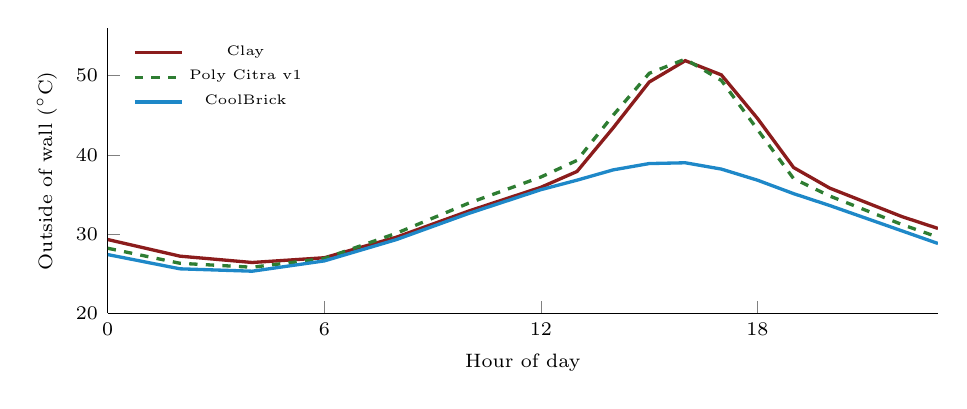
\begin{tikzpicture}
\begin{axis}[width=\linewidth,height=5.2cm,xmin=0,xmax=23,ymin=20,ymax=56,xtick={0,6,12,18},
  xlabel={Hour of day},ylabel={Outside of wall (\si{\celsius})},label style={font=\scriptsize},tick label style={font=\scriptsize},
  legend style={font=\tiny,at={(0.02,0.98)},anchor=north west,draw=none},axis lines*=left]
\addplot[heat!70!black,very thick] coordinates {(0,29.3)(2,27.2)(4,26.4)(6,27)(8,29.6)(10,32.9)(12,35.9)(13,37.9)(14,43.4)(15,49.2)(16,51.9)(17,50.1)(18,44.6)(19,38.4)(20,35.8)(22,32.2)(23,30.7)};\addlegendentry{Clay}
\addplot[leaf,very thick,dashed] coordinates {(0,28.2)(2,26.3)(4,25.8)(6,26.9)(8,30.1)(10,33.9)(12,37.2)(13,39.3)(14,45)(15,50.3)(16,52.1)(17,49.4)(18,43.2)(19,37)(20,34.8)(22,31.2)(23,29.6)};\addlegendentry{Poly Citra v1}
\addplot[sky,very thick] coordinates {(0,27.4)(2,25.6)(4,25.3)(6,26.6)(8,29.3)(10,32.6)(12,35.6)(13,36.8)(14,38.1)(15,38.9)(16,39)(17,38.2)(18,36.8)(19,35.1)(20,33.6)(22,30.4)(23,28.8)};\addlegendentry{CoolBrick}
\end{axis}
\end{tikzpicture}
\column{0.42\textwidth}
\small
\begin{tabular}{@{}lccc@{}}
\toprule
 & Clay & v1 & \textbf{Cool} \\
\midrule
Hottest wall surface & \SI{52}{\celsius} & \SI{52}{\celsius} & \textbf{\SI{39}{\celsius}} \\
Heat let in & 100\% & 32\% & \textbf{17\%} \\
\bottomrule
\end{tabular}

\medskip
The white coat keeps the wall \SI{13}{\celsius} cooler; the air pockets slow the heat.
\textbf{About 80\% less heat} than clay. Real bricks must still be tested.
\end{columns}
\end{frame}

\begin{frame}{Replacing coconut oil}
\begin{columns}[T]
\column{0.52\textwidth}
Our first design used coconut oil to soak up heat, but it was half the cost. The simulation showed it hardly helped: it melts at \SI{27}{\celsius}, and a hot classroom stays above that even at night, so it never sets again.

\medskip
We chose \textbf{Glauber's salt}: very cheap, does not burn, melts at \SI{32}{\celsius}. A little borax and a thickener stop it separating; the pockets are sealed.
\column{0.44\textwidth}
\small
\begin{tabular}{@{}lccc@{}}
\toprule
Filler & Melts & Stores & \rupeesym/brick \\
\midrule
Coconut oil & \SI{27}{\celsius} & 1$\times$ & 35--50 \\
Calcium chloride & \SI{29}{\celsius} & 3$\times$ & 3--8 \\
\textbf{Glauber's salt} & \textbf{\SI{32}{\celsius}} & \textbf{4$\times$} & \textbf{3} \\
\bottomrule
\end{tabular}
\end{columns}
\end{frame}

\begin{frame}{Will it be strong enough?}
\begin{columns}[T]
\column{0.48\textwidth}
\small
\begin{tabular}{@{}lr@{}}
\toprule
 & N/mm\textsuperscript{2} \\
\midrule
Indian standard, lowest class (IS 1077) & $\ge 3.5$ \\
Sand + dissolved Styrofoam (studies) & 4--12 \\
Sand + melted plastic (studies) & 9--33 \\
\bottomrule
\end{tabular}

\medskip
So it can pass. A 190\,mm $\times$ 90\,mm face must hold about \SI{60}{kN} (6 tonnes).
\column{0.48\textwidth}
\small
\textbf{Risks and fixes}
\begin{itemize}
  \item More air pockets $\rightarrow$ weaker: keep walls between pockets thick.
  \item Leftover limonene $\rightarrow$ soft: dry until weight stops dropping.
  \item Fire: add sand and charcoal, plaster both sides.
  \item Sunlight: the white coat protects the plastic.
\end{itemize}
\textbf{Plan:} 3 mixes $\times$ 5 bricks, crushed at a cement-testing lab \todo{lab}.
\end{columns}
\end{frame}

\begin{frame}{Cost: about \rupeesym29 per brick}
\begin{columns}[T]
\column{0.5\textwidth}
\small
\begin{tabular}{@{}lr@{}}
\toprule
Item & \rupeesym \\
\midrule
D-limonene lost while curing & 8.3 \\
Labour (\rupeesym600/day, 150 bricks) & 4 \\
Energy & 4 \\
Styrofoam collection & 3 \\
Glauber's salt + sealing & 5 \\
Sand, charcoal, coat, mould & 4.3 \\
\midrule
\textbf{Total} & \textbf{about 29} \\
\bottomrule
\end{tabular}
\column{0.46\textwidth}
\begin{itemize}
  \item Down from \rupeesym67 in our first design.
  \item Salt instead of coconut oil, and 90\% of the limonene caught and reused.
  \item Best on the sunniest walls.
  \item Funding: Samagra Shiksha school grants, CSR funds, state heat action plans.
\end{itemize}
\end{columns}
\end{frame}

\begin{frame}{UN Sustainable Development Goals}
\begin{columns}[T]
\column{0.24\textwidth}\begin{card}{heat}\textbf{SDG 4}\\ Cooler classrooms help students learn.\end{card}
\column{0.24\textwidth}\begin{card}{citrus}\textbf{SDG 11}\\ Greener buildings from local waste.\end{card}
\column{0.24\textwidth}\begin{card}{leaf!70!black}\textbf{SDG 12}\\ Styrofoam and peel reused, not dumped.\end{card}
\column{0.24\textwidth}\begin{card}{leaf}\textbf{SDG 13}\\ No kiln emissions; cope better with heatwaves.\end{card}
\end{columns}
\end{frame}

\begin{frame}{Next steps}
\begin{enumerate}
  \item Crush-test three mixes; test water, heat and fire safety.
  \item Make and seal the salt pockets; check they do not leak.
  \item Build the two model rooms and log temperatures for 30 days.
  \item Build a test wall at a government school (with permission).
  \item Work with local builders and NGOs to make bricks at scale.
\end{enumerate}
\end{frame}

\begin{frame}{v1 vs v2}
\small
\begin{tabularx}{\textwidth}{@{}lXX@{}}
\toprule
 & Version 1 & CoolBrick (v2) \\
\midrule
Purpose & Turn two wastes into a brick & Also keep buildings cool \\
Inside & Solid & Air pockets, salt pockets, peel charcoal \\
Outside & Plain & White coat that reflects sunlight \\
Heat let in (clay = 100\%) & 32\% & 17\% \\
Solvent & Used once & 90\% recovered and reused \\
Cost per brick & --- & about \rupeesym29 \\
\bottomrule
\end{tabularx}
\end{frame}

\begin{frame}{References}
\tiny
\begin{enumerate}
\item Park, Goodman, Hurwitz \& Smith (2020). Heat and Learning. \emph{AEJ: Economic Policy} 12(2).
\item Ministry of Education (2024). UDISE+ 2023--24.
\item Li et al.\ (2020). Sub-ambient radiative cooling paints. \emph{Cell Reports Physical Science} 1(10).
\item Florida Chemical Co.\ D-limonene as a solvent for EPS; Sony limonene EPS recycling system.
\item EPS mortar with dissolved-foam binder, TNI Journal (ThaiJO); EPS-in-gasoline binder, ASCE J.\ Mater.\ Civ.\ Eng.
\item Plastic-sand bricks, J.\ Univ.\ Babylon; HDPE-sand bricks with kaolin, DUT; waste-plastic masonry in fire, Stellenbosch.
\item ORNL review of low-cost PCMs; CMC-thickened Glauber's salt, \emph{Materials} 17(10) 2442 (2024).
\item Bureau of Indian Standards: IS 1077, IS 3495. United Nations (2015) 2030 Agenda.
\end{enumerate}
\end{frame}

\begin{frame}[standout]
Thank you\\[6pt]
{\normalsize Rian Sikka \& Daiwik Abrol}
\end{frame}

\end{document}
